
\documentclass[a4paper,11pt]{article}
\usepackage{a4wide}
\usepackage{fullpage}
\usepackage[utf8x]{inputenc}
\usepackage[slovene]{babel}
\selectlanguage{slovene}
\usepackage[toc,page]{appendix}
\usepackage[pdftex]{graphicx} % za slike
\usepackage{setspace}
\usepackage{color}
\definecolor{light-gray}{gray}{0.95}
\usepackage{listings} % za vključevanje kode
\usepackage{hyperref}
\renewcommand{\baselinestretch}{1.2} % za boljšo berljivost večji razmak
\renewcommand{\appendixpagename}{Priloge}

\lstset{ % nastavitve za izpis kode, sem lahko tudi kaj dodaš/spremeniš
language=Python,
basicstyle=\footnotesize,
basicstyle=\ttfamily\footnotesize\setstretch{1},
backgroundcolor=\color{light-gray},
}

\title{Podobnost jezikov}
\author{Tomaž Tomažič(63100281)}
\date{\today}

\begin{document}

\maketitle

\section{Uvod}

Cilj naloge je ugotoviti, kateri jeziki so si blizu in narediti program, ki z neko verjetnostjo določi jezik priložene datoteke.

\section{Podatki}

Nalogi je bilo podano 263 datotek z vsebino 'Splošna deklaracija človekovih pravic' v različnih jezikih. Za uspešno rešitev naloge, je bilo potrebno izbrati 20 različnih jezikov in najti še perzijski prevod, ki ga nikakor nisem mogel poiskati z brskalnikom google. Zato sem si za perzijski prevod pomagal s spletno aplikacijo google translate. Čeprav vem, da tak način prevajanja ni 100\% pravilen, sem se za to rešitev vseeno odločil, ker so take besede pravilno prevedene vendar ne nujno v pravilnem vrstnem redu, kar nima zelo velikega vpliva za podano nalogo.

\section{Metode}

Potrebno izgradnjo hierarhije jezikov, sem naredil po principu povprečne razdalje (ang. average linkage). Za računanje razdalj sem uporabil kosinusno podobnost. 
Formula za podobnost je: 
\begin{equation} 
podobnost(X,Y)= 
\frac{X\cdot Y}
{||X|| ||Y||} 
\end{equation} 
Funkcija ki implementira kosinusno podobnost (cosDist), sprejme 2 argumenta X in Y. Argumenta sta slovar, katerega ključ je par znakov, vrednost pa število pojavitev tega para črk v izbranem besedilu. Za lažje računanje frekvenc poskrbi metoda frequency. Način s katero program oceni verjetnost podanega jezika deluje tako, da primerja podani jezik z vsemi ostalimi in izračuna kosinusno razdaljo. Vse razadlje sešteje in normalizira, da lahko izpiše verjetnosti. Tak način ni v vseh primerih najboljši, saj je verjetnost linearno določena, kar pa ni vedno res.
Prikaz hierarhije jezikov sem naredil z izrisom dendrograma~\ref{slika1}. Za izris dendrograma sem potreboval še ostale metode: drawdendrogram, getheight, getdepth in drawnode. Te sem prepisal iz knjige Programming Collective Intelligence in jih preuredil za moje potrebe.

\begin{figure}[htbp]
\begin{center}
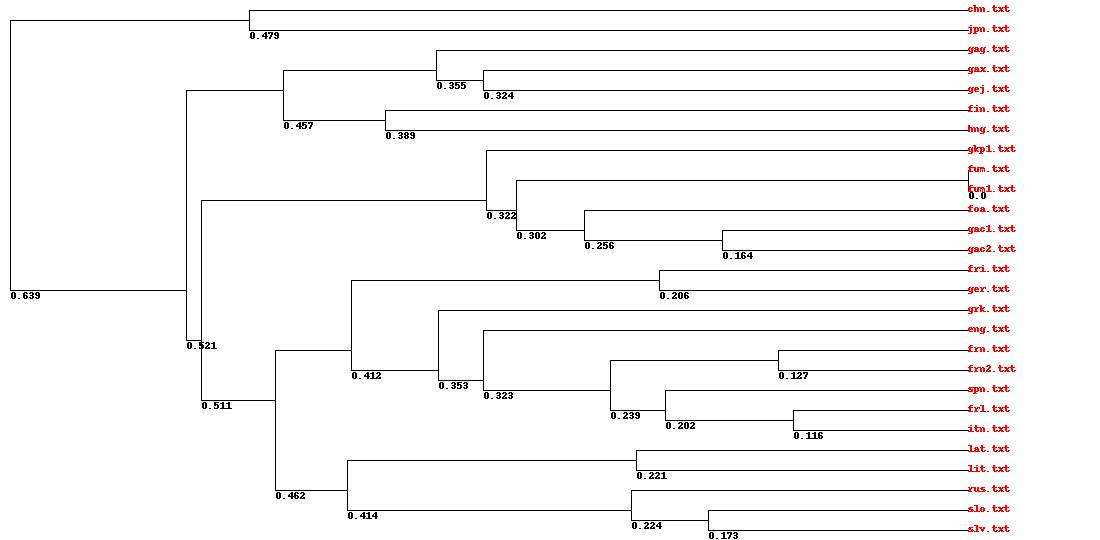
\includegraphics[scale=0.4]{languageGroup-dendrogram.jpg}
\caption{Prikaz hierarhije podobnosti izbranih jezikov}
\label{slika1}
\end{center}
\end{figure}

\section{Rezultati}

\subsection{Hierarhija jezikov}
Iz dendrograma je razvidno, da so si nekateri jeziki lahko bolj podobni kot drugi, ne glede na pisavo. Vhodno bazo podatkov sem izbral tako, da sem lahko že prej predvideval, kateri jeziki so si podobni. Svoje hipoteze sem potrdil s podobnostjo jezikov med Rusijo, Slovenijo in Slovaško; Italjanščino, Francoščino Španščino; Latvijščino in Litovščino; ...
\subsection{Ugotavljanje jezika}
Ugotavljanje jezika na tako preprost način, je izjemno zanimivo in učinkovito. Že z nekaj stavki program pravilno pove, v katerem jeziku je naša vhodna datoteka 
\subsection{Primerjanje 2 razdalj (dodatno)}
Podobnost med finščino in madžarščino ni taka kot med angleščino in perziščino. Med finščino in madžarščino program izračuna razdaljo 0.389, med angleščino in perziščino pa 0.663. Iz tega ne morem sklepati, da sta si jezika blizu. 

\section{Izjava o izdelavi domače naloge}
Domačo nalogo in pripadajoče programe sem izdelal sam.


\end{document}
